\counterwithin{figure}{chapter}			%e.g: Figure 1.1
\counterwithout{table}{chapter}		 	%1 --- сквозная нумерация по всей диссертации
\chapter{First chapter}
\label{ch:ch1}

\begin{figure}
    \centering
    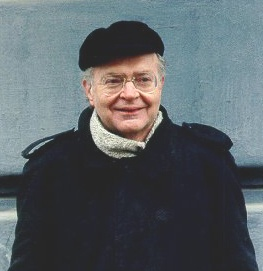
\includegraphics[width=0.4\linewidth]{images/knuth}
    \caption{Knuth}
    \label{fig:my_label4}
\end{figure}


\section{Refs}

\cite{KKK, Gerasimov2023a, Gerasimov2023b, NikGerbook2022}


\section{Units}\label{sec:units}
Числа форматируются при помощи команды \verb|\num|:
\num{5,3};
\num{2,3e8};
\num{12345,67890};
\num{2,6 d4};
\num{1+-2i};
\num{.3e45};
\num[exponent-base=2]{5 e64};
\num[exponent-base=2,exponent-to-prefix]{5 e64};
\num{1.654 x 2.34 x 3.430}
\num{1 2 x 3 / 4}.


Обратите внимание, что ГОСТ запрещает использование знака <<->> для обозначения отрицательных чисел
за исключением формул, таблиц и~рисунков.
Вместо него следует использовать слово <<минус>>.

Размерности можно записывать при помощи команд \verb|\si| и \verb|\SI|:
\si{\farad\squared\lumen\candela};
\si{\joule\per\mole\per\kelvin};
\si[per-mode = symbol-or-fraction]{\joule\per\mole\per\kelvin};
\si{\metre\per\second\squared};
\SI{0.10(5)}{\neper};
\SI{1.2-3i e5}{\joule\per\mole\per\kelvin};
\SIlist{1;2;3;4}{\tesla};
\SIrange{50}{100}{\volt}.

\begin{table}
	\centering
	\captionsetup{justification=centering} % выравнивание подписи по-центру
	\caption{Basic SI quantities}%\label{tab:unit:base}
	\begin{tabular}{llc}
		\toprule
		Name 	& 	Command 	& 	Symbol        \\
		\midrule
		Ampere 	 & \verb|\ampere| 	&\si{\ampere}\\
		Candela  & \verb|\candela| 	& \si{\candela} \\
		Kelvin 	 & \verb|\kelvin| 	&\si{\kelvin}\\
		Kilogram & \verb|\kilogram| & \si{\kilogram} \\
		Meter 	 & \verb|\metre| 	&\si{\metre}\\
		Mole 	 & \verb|\mole| 	&\si{\mole}\\
		Second 	 & \verb|\second| 	&\si{\second}\\
		\bottomrule
	\end{tabular}
\end{table}

